\documentclass[11pt,a4paper]{article}
\usepackage[T1]{fontenc}
\usepackage[utf8]{inputenc}
\usepackage{lmodern}
\usepackage[margin=25mm]{geometry}
\usepackage{graphicx,booktabs,longtable,amsmath,microtype,xcolor}
\usepackage[authoryear,round]{natbib}
\usepackage[hidelinks]{hyperref}
\graphicspath{{../figures/}}
% Generated by the analysis. Do not edit.
\newcommand{\nRanges}{6}
\newcommand{\nDivisions}{41}
\newcommand{\nSubbasins}{180}
\newcommand{\domainKm}{3{,}352{,}481}
\newcommand{\rangesDone}{Hindu Kush, Karakoram}
\newcommand{\nRangesDone}{2}
\newcommand{\nUnits}{23}
\newcommand{\nUnitsSig}{0}
\newcommand{\nUnitsRaw}{0}
\newcommand{\nDriverSig}{3}
\newcommand{\slopeHinduKush}{-1.9}
\newcommand{\pHinduKush}{0.29}
\newcommand{\meanHinduKush}{56}
\newcommand{\slopeKarakoram}{3.9}
\newcommand{\pKarakoram}{0.60}
\newcommand{\meanKarakoram}{140}
\newcommand{\kmStable}{244{,}667}
\newcommand{\kmGain}{0}
\newcommand{\kmLoss}{0}
\newcommand{\kmPersistent}{5{,}702}
\newcommand{\kmNodata}{16{,}678}
\newcommand{\kmRare}{115{,}684}
\newcommand{\kmClassified}{382{,}733}

\title{Snow cover change across the Third Pole by mountain division and sub-basin:\\ methods and preliminary results}
\author{Ahmad Ammar}
\date{Working document, regenerated from the analysis}
\begin{document}
\maketitle

\begin{abstract}
This document records how snow cover change is being measured across the mountains of the Third Pole, and what the results show so far. Every number, table and figure is produced by the analysis scripts. Results currently cover \nRangesDone{} of \nRanges{} ranges (\rangesDone{}) and are preliminary.
\end{abstract}

\section{Why this region}
The mountains of High Mountain Asia store and release water for some of the most populous river basins on Earth \citep{Immerzeel_2010,Immerzeel_2019,Wester_2019}. Seasonal snow matters as much as glacier ice in much of this supply, particularly in the west, where winter precipitation from western disturbances dominates \citep{Bookhagen_2010,Dimri_2015,Kraaijenbrink_2021}. The Karakoram is a particular puzzle, as its glaciers have changed less than those of neighbouring ranges \citep{Hewitt_2005,Gardelle_2012,Farinotti_2020}.

Earlier studies differ in period, boundary and cloud treatment, so their trends are hard to compare \citep{Maskey_2011,Gurung_2017,Hasson_2014,Notarnicola_2020}. ICIMOD has also released an improved MODIS product for this region, which reduces cloud and sensor errors \citep{Muhammad_2020}, and this work will be compared with it. The contribution here is a single, openly reproducible comparison across fixed mountain and river units.

\section{Regions}
Ranges and divisions follow the GMBA Mountain Inventory v2 \citep{Snethlage_2022}, and sub-basins follow HydroBASINS level 5 \citep{Lehner_2013}, clipped to those mountains. This gives \nRanges{} ranges, \nDivisions{} divisions and \nSubbasins{} sub-basins over \domainKm{}~km$^2$ (Figure~\ref{fig:regions}). The mountain definition excludes flat plateau interiors, so results describe mountain terrain and not the whole plateau.

\begin{figure}[htbp]\centering
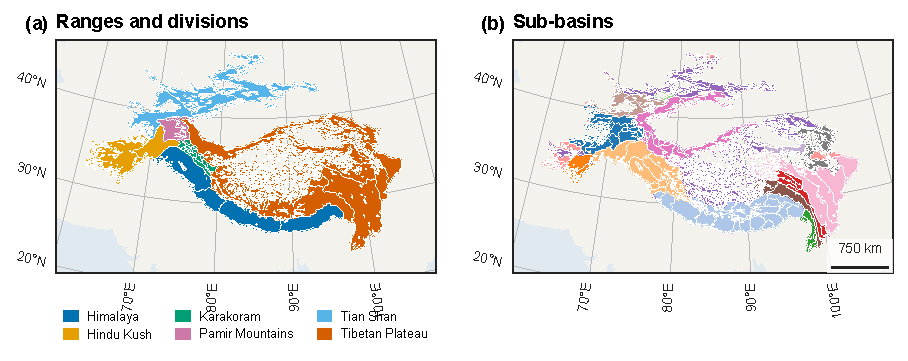
\includegraphics[width=\textwidth]{fig_regions.pdf}
\caption{Analysis units, in an Albers equal-area conic projection with standard parallels at 25$^\circ$N and 45$^\circ$N. The scale bar is true along those parallels. Boundaries imply no position on any territorial claim.}\label{fig:regions}
\end{figure}

\section{Data and methods}
\paragraph{Snow.} Daily MOD10A1 collection 6.1 \citep{Hall_2002,Riggs_2017} gives NDSI snow cover at 500~m. A clear pixel with NDSI snow cover of at least 40 counts as snow; this threshold is still to be tested against alternatives. For each hydrological year (October to September), duration is $365 \times$ snow days $/$ clear days, for pixels with at least 120 clear days. Scaling by clear days assumes that cloudy days resemble clear ones, which is a known weakness to be tested against gap filling and the Aqua sensor.

\paragraph{Pixel classes.} Each pixel with at least 20 usable years is tested with Mann-Kendall \citep{Yue_2002}, with false discovery control at 5\% \citep{Benjamini_1995,Wilks_2016}. Significant pixels are gain or loss. Others are `no detectable trend' or `rarely snow' (under 15 days a year). Pixels snow-covered on at least 80\% of clear days from 1 August to 15 September are `persistent snow or ice', split by GLIMS glacier outlines. MODIS cannot separate snow from ice, and persistence does not measure glacier health; that needs mass-balance estimates such as \citet{Hugonnet_2021}.

\paragraph{Unit trends.} Annual means per unit use the Sen slope \citep{Sen_1968}. The quoted $p$ is the larger of the plain Mann-Kendall test and trend-free pre-whitening, and $q$ applies false discovery control across units. The Hamed-Rao correction \citep{Hamed_1998} was tried and rejected, because it gave near-zero $p$ for very weak trends in these 25-value series.

\paragraph{Climate.} Temperature, precipitation and snowfall come from ERA5-Land \citep{MunozSabater_2021}, whose accuracy at altitude is limited \citep{Palazzi_2013}. Nino 3.4, the dipole mode index \citep{Saji_1999} and South Asian monsoon rainfall come from a companion analysis and have not yet been independently reviewed. Series are detrended and compared by Spearman correlation. These are associations and do not establish causes.

\section{Preliminary results}
Of \kmClassified{}~km$^2$ classified so far, \kmStable{}~km$^2$ show no detectable trend, \kmGain{}~km$^2$ show gain, \kmLoss{}~km$^2$ show loss, \kmPersistent{}~km$^2$ are persistent, \kmRare{}~km$^2$ rarely have snow, and \kmNodata{}~km$^2$ lack enough clear days (Figure~\ref{fig:classes}). `No detectable trend' does not establish stability, as 25 years gives limited power at pixel level.

Across \nUnits{} units, \nUnitsRaw{} have $p<0.05$ and \nUnitsSig{} remain after false discovery control (Table~\ref{tab:trends}, Figures~\ref{fig:series} and \ref{fig:heat}). Of the climate associations tested, \nDriverSig{} remain after false discovery control (Figure~\ref{fig:attr}).

\begin{figure}[htbp]\centering
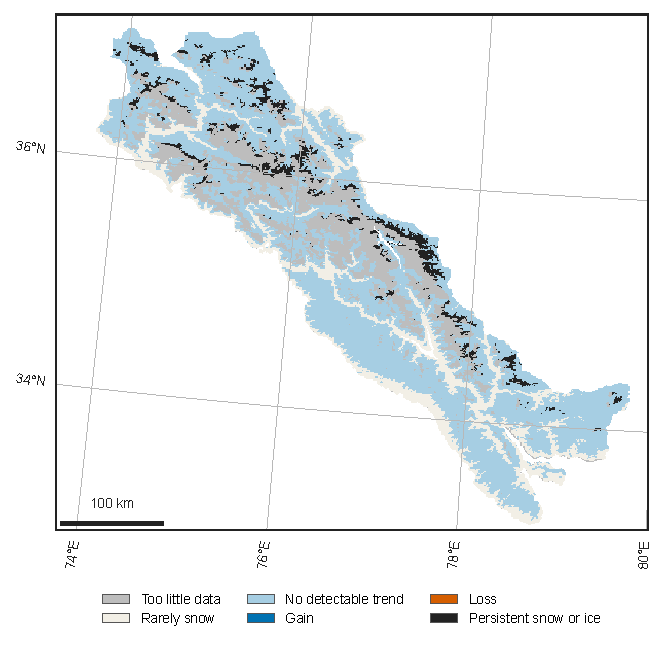
\includegraphics[width=\textwidth]{fig_change_classes.pdf}
\caption{Snow cover change classes, 2001--2025, resampled to 1~km by nearest pixel for display. Preliminary.}\label{fig:classes}
\end{figure}

\begin{figure}[htbp]\centering
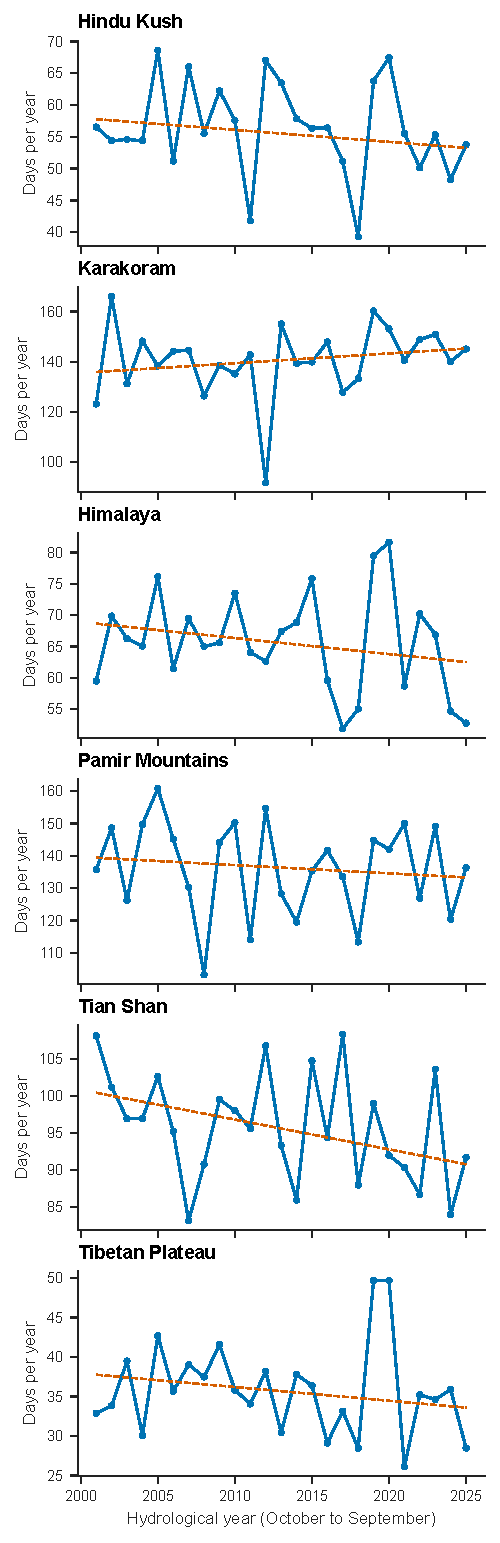
\includegraphics[width=0.6\textwidth]{fig_series.pdf}
\caption{Mean snow-cover duration by range, with Sen slope (dashed). Preliminary.}\label{fig:series}
\end{figure}

\begin{figure}[htbp]\centering
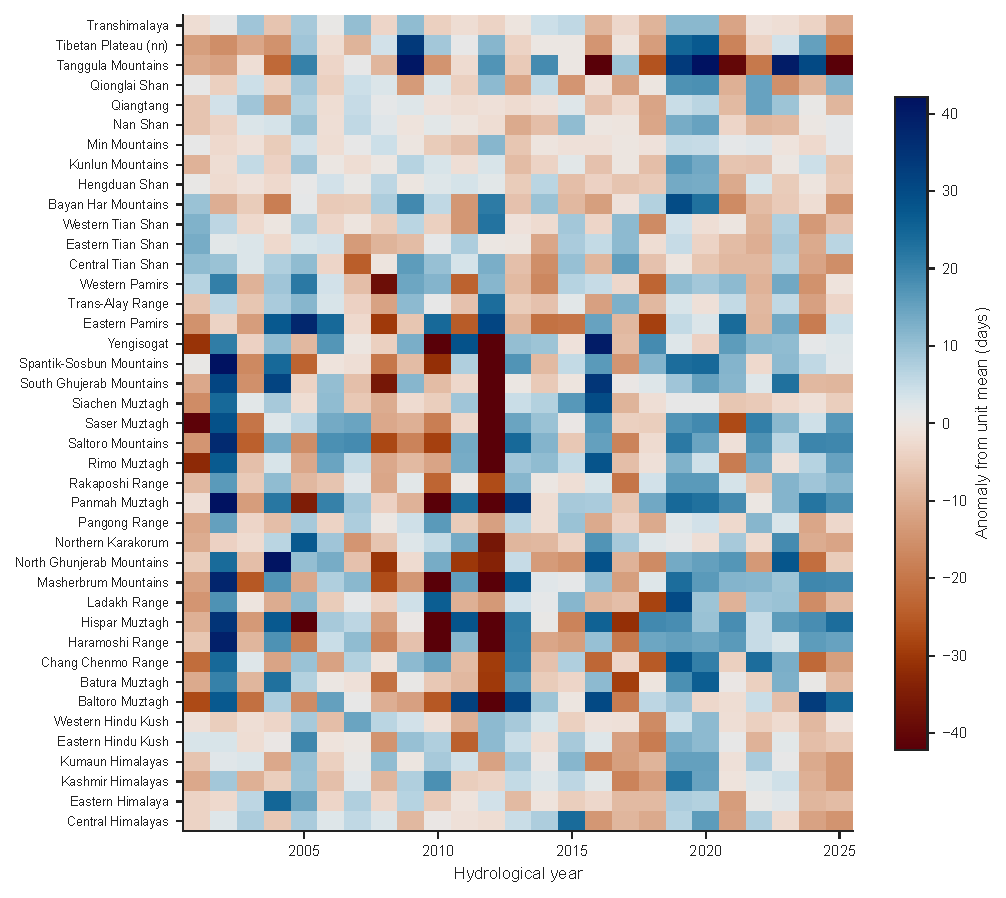
\includegraphics[width=\textwidth]{fig_anomaly_heatmap.pdf}
\caption{Duration anomaly by division and year, on a perceptually uniform diverging colour map \citep{Crameri_2020}. Preliminary.}\label{fig:heat}
\end{figure}

\begin{figure}[htbp]\centering
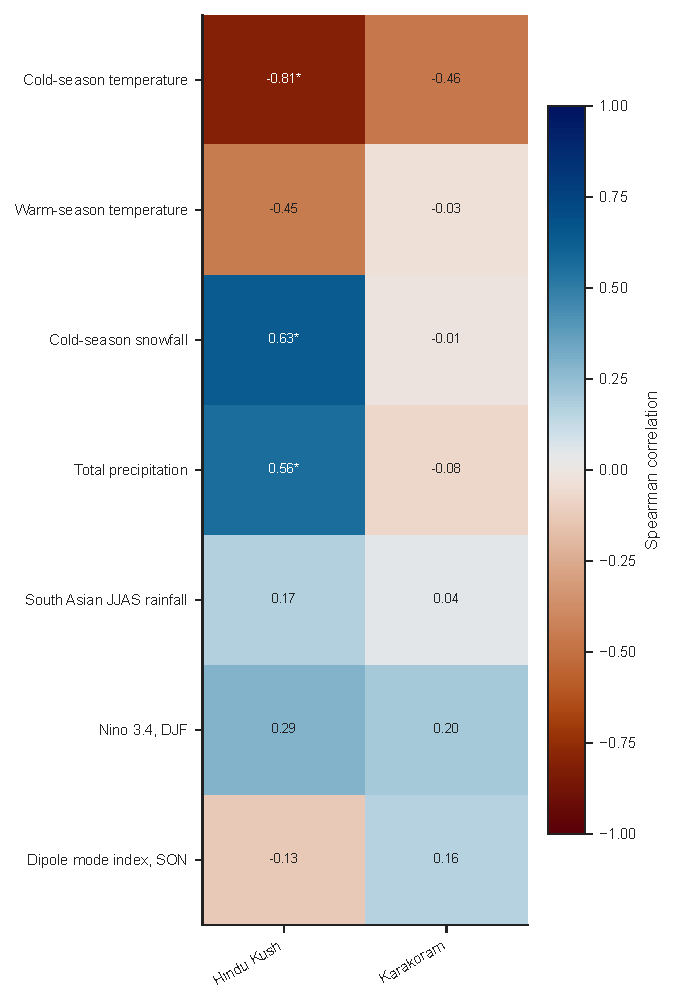
\includegraphics[width=0.7\textwidth]{fig_attribution.pdf}
\caption{Spearman correlation of detrended duration with climate series. An asterisk marks $q<0.05$. Preliminary.}\label{fig:attr}
\end{figure}

\begin{table}[htbp]\centering\scriptsize
\caption{Trends in snow-cover duration, 2001--2025. Preliminary.}\label{tab:trends}
\begin{tabular}{llrrrrr}
\toprule
Unit & Parent & Area (km$^2$) & Mean (days) & Sen slope (days per decade) & $p$ & $q$ \\
\midrule
Tibetan Plateau & -- & 1{,}759{,}351 & 36 & -1.7 & 0.315 & 0.986 \\
Tian Shan & -- & 560{,}184 & 96 & -4.0 & 0.172 & 0.986 \\
Himalaya & -- & 555{,}855 & 66 & -2.6 & 0.388 & 0.986 \\
Hindu Kush & -- & 308{,}130 & 56 & -1.9 & 0.293 & 0.986 \\
Pamir Mountains & -- & 94{,}347 & 136 & -2.5 & 0.637 & 0.986 \\
Karakoram & -- & 74{,}614 & 140 & +3.9 & 0.602 & 0.986 \\
Kashmir Himalayas & Himalaya & 183{,}700 & 100 & -0.0 & 1.000 & 1.000 \\
Central Himalayas & Himalaya & 161{,}140 & 44 & -3.8 & 0.168 & 0.986 \\
Eastern Himalaya & Himalaya & 142{,}951 & 34 & -3.6 & 0.072 & 0.986 \\
Kumaun Himalayas & Himalaya & 68{,}064 & 59 & -1.1 & 0.761 & 0.986 \\
Western Hindu Kush & Hindu Kush & 201{,}904 & 32 & -1.5 & 0.559 & 0.986 \\
Eastern Hindu Kush & Hindu Kush & 106{,}225 & 102 & -2.8 & 0.602 & 0.986 \\
Ladakh Range & Karakoram & 13{,}681 & 95 & -0.5 & 0.907 & 0.986 \\
Chang Chenmo Range & Karakoram & 8{,}940 & 101 & +0.6 & 0.944 & 0.986 \\
Batura Muztagh & Karakoram & 7{,}136 & 168 & +1.5 & 0.785 & 0.986 \\
Saltoro Mountains & Karakoram & 5{,}506 & 150 & +6.5 & 0.216 & 0.986 \\
Masherbrum Mountains & Karakoram & 4{,}835 & 123 & +9.9 & 0.129 & 0.986 \\
Saser Muztagh & Karakoram & 4{,}355 & 160 & +6.9 & 0.442 & 0.986 \\
North Ghunjerab Mountains & Karakoram & 4{,}024 & 206 & -2.5 & 0.797 & 0.986 \\
South Ghujerab Mountains & Karakoram & 3{,}747 & 178 & +4.1 & 0.710 & 0.986 \\
Baltoro Muztagh & Karakoram & 2{,}920 & 188 & +8.4 & 0.535 & 0.986 \\
Hispar Muztagh & Karakoram & 2{,}868 & 195 & +8.1 & 0.441 & 0.986 \\
Haramoshi Range & Karakoram & 2{,}744 & 120 & +4.7 & 0.315 & 0.986 \\
Rimo Muztagh & Karakoram & 2{,}284 & 231 & +5.2 & 0.941 & 0.986 \\
Spantik-Sosbun Mountains & Karakoram & 2{,}164 & 182 & +6.5 & 0.414 & 0.986 \\
Rakaposhi Range & Karakoram & 2{,}051 & 108 & +6.1 & 0.172 & 0.986 \\
Northern Karakorum & Karakoram & 1{,}881 & 92 & +0.3 & 0.944 & 0.986 \\
Yengisogat & Karakoram & 1{,}659 & 184 & +2.5 & 0.528 & 0.986 \\
Pangong Range & Karakoram & 1{,}533 & 42 & -0.8 & 0.761 & 0.986 \\
Siachen Muztagh & Karakoram & 1{,}392 & 260 & -1.8 & 0.559 & 0.986 \\
Panmah Muztagh & Karakoram & 890 & 208 & +6.2 & 0.338 & 0.986 \\
Western Pamirs & Pamir Mountains & 57{,}954 & 160 & -3.0 & 0.568 & 0.986 \\
Eastern Pamirs & Pamir Mountains & 24{,}626 & 90 & -1.7 & 0.761 & 0.986 \\
Trans-Alay Range & Pamir Mountains & 11{,}768 & 115 & -1.5 & 0.441 & 0.986 \\
Eastern Tian Shan & Tian Shan & 219{,}243 & 96 & -1.6 & 0.862 & 0.986 \\
Western Tian Shan & Tian Shan & 172{,}359 & 82 & -3.2 & 0.189 & 0.986 \\
Central Tian Shan & Tian Shan & 168{,}581 & 110 & -7.1 & 0.050 & 0.986 \\
Transhimalaya & Tibetan Plateau & 413{,}137 & 38 & -2.7 & 0.199 & 0.986 \\
Hengduan Shan & Tibetan Plateau & 386{,}527 & 24 & -1.3 & 0.472 & 0.986 \\
Kunlun Mountains & Tibetan Plateau & 278{,}969 & 52 & -0.1 & 0.981 & 1.000 \\
Nan Shan & Tibetan Plateau & 193{,}515 & 29 & -1.1 & 0.624 & 0.986 \\
Qiangtang & Tibetan Plateau & 184{,}291 & 31 & -0.6 & 0.691 & 0.986 \\
Bayan Har Mountains & Tibetan Plateau & 107{,}306 & 41 & -0.3 & 0.870 & 0.986 \\
Min Mountains & Tibetan Plateau & 94{,}198 & 13 & +0.9 & 0.315 & 0.986 \\
Qionglai Shan & Tibetan Plateau & 53{,}220 & 40 & +0.6 & 0.907 & 0.986 \\
Tanggula Mountains & Tibetan Plateau & 40{,}763 & 80 & +5.3 & 0.710 & 0.986 \\
Tibetan Plateau (nn) & Tibetan Plateau & 7{,}239 & 30 & +3.5 & 0.747 & 0.986 \\
\bottomrule
\end{tabular}

\end{table}

\section{Harmonisation}
Studies of this region are hard to combine because they use different boundaries, periods and units. Every dataset in this project therefore follows one standard, so that others can add to it.

\begin{itemize}
\item \textbf{Space.} Vector files are GeoJSON in WGS~84. Each region has a stable identifier (GMBA or HydroBASINS) and a boundary version. Areas are computed in an equal-area projection, never in degrees.
\item \textbf{Time.} Years are hydrological, October to September, named by the year in which they end. Dates are ISO~8601.
\item \textbf{Tables.} Long form, one row per unit and period, with explicit units in column names (for example \texttt{km2}, \texttt{days}, \texttt{mm}), and missing values left empty.
\item \textbf{Rasters.} Native grid retained, with resampling recorded whenever it happens.
\item \textbf{Provenance.} Each file records its source, product version, licence, script and date, in a catalogue. Originals stay read-only and are hashed.
\item \textbf{Names.} A file name says what the file holds. Numbers mean a year or a version, never the order of saving.
\end{itemize}

The same standard will be applied in turn to glacier outlines and mass balance \citep{Hugonnet_2021}, climate series, and the monsoon indices.

\section{Further checks}
\paragraph{Himalayan loss.} Loss pixels lie mostly in the Eastern and Central Himalaya, next to the cloudiest ground. Following those pixels through 2003--2025 gives $\lossTerra{}$~days per decade in Terra, $\lossAqua{}$ in Aqua, and $\lossMerged{}$ with the two combined. It holds at thresholds of 30, 40 and 50. Clear days show no significant trend ($p=\clearTerraP{}$ and $\clearAquaP{}$). So changing cloud does not explain it. The pixels were chosen because Terra showed loss, so these rates overstate the typical pixel, and Aqua sees the same snow. Landsat or Sentinel-2 remain the proper independent test.

\paragraph{Sub-basins.} Of \nSub{} sub-basins, \nSubRaw{} have $p<0.05$ and \nSubSig{} remain after correction. About nine would be expected by chance.

\section{Method log}
Decisions that changed results, newest last. Reasons are kept so that the same mistakes are not repeated.
\begin{enumerate}
\item Rectangular ranges replaced by GMBA divisions and HydroBASINS sub-basins.
\item Hamed-Rao correction dropped: it gave near-zero $p$ for very weak trends in 25 values.
\item False discovery threshold refined: bins of 0.0005 returned zero wrongly; bins of one millionth do not.
\item The Tibetan Plateau tested at 500~m by batch, after timing out interactively, since a test at 1~km had found nothing.
\item Literature search showed regional trend papers exist (see \texttt{gap\_analysis}), so the main question moves to why published trends disagree, and what can be detected.
\end{enumerate}

\section{Still to do}
Complete the remaining ranges and the sub-basins; test the NDSI threshold, Aqua and gap filling; investigate the 2012 low in the Karakoram, where daily images are complete and a smaller dip also appears in MOD10A2; compare with MOYDGL06 \citep{Muhammad_2020}; validate against Landsat, Sentinel-2 and stations; and review the climate indices.

\bibliographystyle{agsm}
\bibliography{../references/refs}
\end{document}
